\begin{abstract}
I study three ways to search binary document vectors after selecting clusters: a full scan,
Bitplanes, and Backward Walk. I compare their work, memory use and retrieval time using the
same documents and queries. The experiments examine when the extra index work saves enough
full document scores to reduce latency at a required recall.
\end{abstract}

\section{Introduction}
\subsection{Exa method and end to end pipeline}
Let's first understand the ``original'' pipeline that I am trying to improve upon.

Note that the architecture I am referring to here is based on the pipeline described in
Exa's article~\cite{exa}. I am aware that Exa's actual production system may have changed or
improved since then, but for the purpose of this report, let's treat the architecture
described in that article as the original baseline that we compare against.

Detail: In this pipeline, document embeddings are first shortened using Matryoshka
representations, converted into binary signs, and assigned to clusters. At query time,
the query is encoded, a subset of nearby clusters is selected, and the documents inside
those clusters are scored using the floating-point query. The top candidates can then be
reranked using the original uncompressed vectors.

The main part that I am trying to improve in this report is the search stage after cluster
selection. The two new approaches introduced later, Bitplanes and Backward Walk, replace
this step while keeping the rest of the pipeline largely the same.

\begin{figure}[H]\centering
\begin{tikzpicture}[node distance=4mm]
\node[box,text width=18mm] (doc) {Document\\text};
\node[box,text width=26mm,right=of doc] (embed) {Matryoshka\\embedding};
\node[box,text width=23mm,right=of embed] (bits) {Keep $d$ values\\and pack signs};
\node[box,text width=30mm,right=of bits] (store) {Assign clusters\\and build index};
\draw[arr](doc)--(embed);\draw[arr](embed)--(bits);\draw[arr](bits)--(store);
\node[box,text width=18mm,below=11mm of doc] (q) {Query text};
\node[box,text width=26mm,right=of q] (qe) {Floating-point\\query};
\node[box,text width=23mm,right=of qe] (route) {Select nearby\\clusters};
\node[box,text width=30mm,draw=ForestGreen!80!black,fill=ForestGreen!14,line width=1.1pt,right=of route] (search) {\textbf{Test A / B / C}\\Search inside\\selected clusters};
\node[box,text width=23mm,right=of search] (rerank) {Rerank using\\full vectors};
\draw[arr](q)--(qe);\draw[arr](qe)--(route);\draw[arr](route)--(search);\draw[arr](search)--(rerank);
\end{tikzpicture}
\caption{Green marks the part we aim to improve: document search inside the selected clusters, using A, B or C. Reranking is shown as a separate step.}
\end{figure}

\subsection{Idea background}
When I took a closer look at the pipeline, one part that particularly stood out to me was
the comparison between the floating-point query and the binary-quantized document.

Consider a simple example:
\[
q=[0.7,\ 0.5,\ -0.4,\ -0.6,\ 0.3]
\]
and suppose a document is represented using binary signs, where 1 means $+1$ and 0 means $-1$.
For example:
\[
\text{Document}=\texttt{11000}
\]
The score is calculated by taking the dot product between the query values and the document
signs. So for \texttt{11000}, the score is
\[
0.7(+1)+0.5(+1)+(-0.4)(-1)+(-0.6)(-1)+0.3(-1)=1.9.
\]
Now, something interesting follows from this. Just by looking at the signs of the query,
we already know what the ideal binary document would look like.

For every positive query value, we would prefer the corresponding document bit to be 1,
and for every negative query value, we would prefer it to be 0. Therefore, for the query
above, the ideal binary pattern is
\[
\texttt{11001}.
\]
This document would achieve the maximum possible score:
\[
0.7+0.5+0.4+0.6+0.3=2.5.
\]
From here, we can think about every other document in terms of how far it is from this ideal
pattern. More importantly, not every mismatch has the same cost. If we mismatch the first
coordinate, where $|q_1|=0.7$, the score decreases by 1.4. But if we mismatch the last
coordinate, where $|q_5|=0.3$, the score only decreases by 0.6.

In more formal terms, let
\[
Q=\sum_i|q_i|
\]
be the score of the ideal binary pattern. If a document $b$ disagrees with the query sign
at some coordinates, define its mismatch penalty as
\[
p=\sum_{i:b_i\ne\operatorname{sign}(q_i)}|q_i|.
\]
Then its score can be written as
\begin{equation}
S(q,b)=Q-2p.
\label{eq:score}
\end{equation}
This observation is the main idea behind the approaches explored in this report. Instead
of treating every binary document equally and scoring all of them one by one, can we use
the query itself to guide the search toward documents that are closer to its ideal binary
pattern, while avoiding unnecessary full-score calculations?

\subsection{Exploring new methods}
From the previous section, we know two useful things before we even start searching:

We know what the ideal binary document looks like from the signs of the query.
We know that some bits matter more than others, based on the magnitude $|q_i|$.

The next question is therefore:

Can we build an index that uses this information directly, instead of treating every
document inside the selected clusters equally?

This led me to explore two approaches.

The first, Bitplanes, starts from a large set of candidate documents and progressively
narrows it down using the query.

The second, Backward Walk, approaches the problem from the opposite direction: it starts
from a very specific binary pattern and progressively relaxes the constraints until enough
useful candidates are found.

\subsubsection{Bitplanes}
Now that we know what the ideal document looks like based on the query, one idea is to
build a data structure that makes filtering by individual bits very cheap.

Normally, binary documents are stored row by row:
\begin{verbatim}
ID 2: 10100
ID 3: 11001
ID 4: 11000
\end{verbatim}
Instead, we can additionally store an inverted representation of the same bits:

\begin{figure}[H]\centering
\begin{tikzpicture}
\node[box,text width=30mm] (q) at (4.7,.25) {$|q|$ priority\\$1\to4\to2\to3\to5$};
\node[align=left,font=\small] (rows) at (0,-2) {Packed documents\\ID 2: \texttt{10100}\\ID 3: \texttt{11001}\\ID 4: \texttt{11000}};
\node[align=center,font=\small] (planes) at (4.7,-2) {\begin{tabular}{c|ccc}
 & ID 2 & ID 3 & ID 4\\\hline
Bit 1 &1&1&1\\
\color{Branch}Bit 2&\color{Branch}0&\color{Branch}1&\color{Branch}1\\
Bit 3&1&0&0\\Bit 4&0&0&0\\Bit 5&0&1&0
\end{tabular}};
\node[branch,text width=38mm] (mask) at (10,-2) {Current: \texttt{111}\\AND bit 2: \texttt{011}\\Result: \texttt{011}};
\draw[arr](rows)--(planes);\draw[arr](planes)--(mask);\draw[arr](q)--(planes);
\end{tikzpicture}
\caption{The same document signs, stored in an extra layout for bitwise filtering.}
\end{figure}

Each row above is what I call a bitplane: one bit position across many documents.

Suppose the query is
\[
q=[0.7,\ 0.5,\ -0.4,\ -0.6,\ 0.3].
\]
From the magnitude of the query values, we can prioritize the bits approximately as
\[
1,\ 4,\ 2,\ 3,\ 5,
\]
because
\[
0.7>0.6>0.5>0.4>0.3.
\]
Now suppose our current candidate mask is
\[
\texttt{111}
\]
meaning that IDs 2, 3 and 4 are all still possible candidates.

For bit 2, the query prefers 1. The corresponding bitplane is
\[
\texttt{011}
\]
so keeping the documents that match the query is simply
\[
\texttt{111}\ \&\ \texttt{011}=\texttt{011}.
\]
We immediately reduce the candidate set to IDs 3 and 4.

This is attractive because the filtering itself consists mostly of bitwise operations,
which modern CPUs can perform very efficiently.

A simplified first version of the idea might therefore look like:

\begin{minipage}{\linewidth}
\begin{lstlisting}[language=Python]
def full_score(query, code):
    return sum(q if bit else -q for q, bit in zip(query, code))


def greedy_search(query, cluster, k, leaf_size):
    order = sorted(range(len(query)), key=lambda i: -abs(query[i]))
    active = cluster.full_mask
    for bit in order:
        plane = cluster.planes[bit]
        preferred = plane if query[bit] >= 0 else ~plane
        active &= preferred
        if active.bit_count() <= leaf_size:
            break

    best = TopK(k)
    for row_id, code in cluster.rows_in_mask(active):
        best.add(row_id, full_score(query, code))
    return best.results()
\end{lstlisting}
\end{minipage}

However, this simple version has a major problem.

\subsubsection*{PROBLEM 1: Greedily following the preferred bits can miss the best document}
Consider:
\[
q=[0.6,\ 0.5,\ 0.4,\ 0.3].
\]
The ideal binary document is \texttt{1111}.

Suppose the database only contains:
\begin{verbatim}
Document A: 0111
Document B: 1000
\end{verbatim}
If we greedily start with the first bit, the query prefers 1. We would therefore keep
Document B and throw away Document A.

But their complete scores are:
\[
S(A)=-0.6+0.5+0.4+0.3=0.6
\]
while
\[
S(B)=0.6-0.5-0.4-0.3=-0.6.
\]
So Document A is actually better.

The problem is that matching one important bit does not guarantee that the remaining bits
will also match.

\textbf{Solution: branching}\par
Instead of discarding the alternative, we keep both branches.

The branch matching the preferred bit receives no additional mismatch penalty. The alternative
branch is still kept, but its penalty increases by $|q_i|$.

We then explore the branches in order of smallest accumulated penalty. This gives us a
recursive search tree rather than one greedy path.

\begin{figure}[H]\centering
\begin{tikzpicture}
\node[branch,text width=43mm] (root) at (0,0) {2 documents\\$p=0$, bound $1.8$};
\node[branch,text width=48mm] (yes) at (-3.3,-1.6) {Bit 1 = 1: document B\\$p=0$, bound $1.8$\\Full score $-0.6$};
\node[box,text width=48mm] (no) at (3.3,-1.6) {Bit 1 = 0: document A\\$p=0.6$, bound $0.6$\\Full score $0.6$};
\draw[arr](root)--(yes);\draw[arr](root)--(no);
\node[align=center,font=\small] at (0,-3.2) {After scoring B, the other bound is $0.6>-0.6$.\\We must explore A; the first choice was not enough.};
\end{tikzpicture}
\caption{Keep the alternative until its score bound proves it cannot improve the result.}
\end{figure}

\textbf{Stopping condition}\par
Recall:
\[
S(q,b)=Q-2p,\qquad Q=\sum_i|q_i|.
\]
If a branch has already accumulated mismatch penalty $p$, any document below it must have
penalty at least $p$.

Therefore,
\[
U_{\rm branch}=Q-2p
\]
is an upper bound on the score of every document inside that branch.

For example, suppose $Q=2.5$ and we are looking for the top two results. We have already
found 2.5 and 1.9, where 1.9 is the current top-2 threshold.

Now consider an unexplored branch with $p=0.5$. Its absolute best possible score is
\[
2.5-2(0.5)=1.5.
\]
Since $1.5<1.9$, nothing inside that branch can enter our current top two. We can safely
discard the entire subtree.

So:
\[
\boxed{Q-2p<\text{current }K\text{th score}\quad\Rightarrow\quad\text{prune branch}}
\]

\begin{figure}[H]\centering
\begin{tikzpicture}
\node[branch,text width=40mm] (best) at (0,0) {Current best two\\2.5 and 1.9};
\node[box,text width=45mm,fill=gray!20,text=gray] (skip) at (6,0) {Waiting branch: $p=0.5$\\Bound $1.5<1.9$: skip};
\draw[arr](best)--node[above=1mm,font=\small,align=center,text width=17mm]{compare\\with 1.9}(skip);
\node[box,fill=gray!15,text=gray,text width=22mm] (left) at (4.6,-1.3) {unvisited rows};
\node[box,fill=gray!15,text=gray,text width=22mm] (right) at (7.4,-1.3) {unvisited rows};
\draw[arr,dashed](skip)--(left);\draw[arr,dashed](skip)--(right);
\end{tikzpicture}
\caption{The whole gray subtree can be skipped because even its best possible score is too low.}
\end{figure}

If the best remaining branch in the queue already fails this test, then every other branch
is worse and the entire search can stop.

The resulting algorithm is approximately:

\begin{minipage}{\linewidth}
\begin{lstlisting}[language=Python]
from heapq import heappop, heappush
from itertools import count


def bitplane_search(query, clusters, k, leaf_size):
    order = sorted(range(len(query)), key=lambda i: -abs(query[i]))
    ideal_score = sum(abs(q) for q in query)
    sequence = count()
    queue = []
    for cluster in clusters:
        if cluster.full_mask:
            heappush(queue, (0, next(sequence), 0,
                            cluster.full_mask, cluster))
    best = TopK(k)
    while queue:
        penalty, _, depth, active, cluster = heappop(queue)
        upper_bound = ideal_score - 2 * penalty
        if best.full() and upper_bound < best.worst_score():
            break
        if active.bit_count() <= leaf_size or depth == len(query):
            for row_id, code in cluster.rows_in_mask(active):
                best.add(row_id, full_score(query, code))
            continue

        bit = order[depth]
        plane = cluster.planes[bit]
        preferred = plane if query[bit] >= 0 else ~plane
        matching = active & preferred
        # Keep the other half too; its remaining bits may be better.
        children = ((matching, 0), (active ^ matching, abs(query[bit])))
        for mask, extra_penalty in children:
            if mask:
                heappush(queue, (penalty + extra_penalty,
                                next(sequence), depth + 1, mask, cluster))
    return best.results()
\end{lstlisting}
\end{minipage}

This is essentially the branch-and-bound Bitplane search used in the current experiments.

\subsubsection*{PROBLEM 2: Bitwise operations are cheap, but the bitmap itself can still be large}
There is another issue.

A bitwise AND sounds almost free, but it is not literally one operation when the cluster
contains thousands or millions of documents.

Suppose one cluster contains 6400 documents. With 64-bit machine words, one bitplane contains
\[
6400/64=100
\]
machine words.

So one split roughly requires us to loop over those 100 words.

Even worse, suppose after several splits only 80 documents remain. The physical mask can
still be 100 words wide. So the next split may still need to process those same 100 words.

\begin{figure}[H]\centering
\begin{tikzpicture}
\node[anchor=west,font=\small] at (0,1.1) {Initial mask: 6400 candidates};
\fill[Branch!65](0,.3) rectangle (12,.75);
\node[anchor=west,font=\small] at (0,-.2) {After filtering: 80 candidates};
\fill[gray!15](0,-1) rectangle (12,-.55);
\foreach \x in {0.3,2.6,6.7,10.8}{\fill[Branch](\x,-1) rectangle +(0.12,.45);}
\draw[<->,Ink](0,-1.5)--node[below,font=\small]{Both masks span 100 machine words}(12,-1.5);
\end{tikzpicture}
\caption{Fewer active document positions do not make this dense mask physically shorter.}
\end{figure}

\textbf{Bitmap traversal cost.} In general, for a cluster containing $n$ documents, one dense
bitplane operation costs roughly $O(\ceil{n/64})$ word operations. If we visit $J$ split
nodes, this becomes approximately $O(J\ceil{n/64})$, before even counting queue operations
and the final document scoring. This was one of the important findings from the earlier
experiments: reducing the number of fully scored documents does not automatically mean
reducing total query time, because the bitmap traversal itself can become expensive.

\textbf{Solution 1: Parameter tuning.} This problem is technically something we can optimize.
For example, we can tune cluster size during coarse routing; number of clusters probed;
how deep we split; leaf size; when we switch back to ordinary full scoring. So Bitplanes
is not fundamentally broken. The question is finding the point where scores avoided are
worth more than additional bitmap traversal.

\textbf{Solution 2: Other approach.} However, thinking about this cost led me to a second idea.
Bitplanes starts with a large set of documents and repeatedly narrows it down. What if we
instead did the opposite? If Bitplanes can be thought of as bottom-up, then Backward Walk
can be thought of as top-down: start from the most specific binary pattern we can describe
and progressively broaden the search only when necessary.

\subsubsection{Backward Walk}
Backward Walk builds on the same observation:

Given a query, we already know what its ideal binary document should look like.

However, instead of starting with thousands of documents and filtering them using bitplanes,
we try to start directly from a small bucket of documents that already looks similar to the query.

Suppose the binary query begins with \texttt{101101001011...}.

Using all 256 bits as a lookup key would be far too specific. With a large binary space,
the probability that an exact 256-bit pattern actually exists in the database is extremely small.

Instead, suppose we choose a prefix length $x$. For example, the first 16 bits:
\[
\texttt{1011010010110101}
\]
During index construction, documents sharing this prefix are placed in the same bucket or
contiguous range.

At query time, we directly look up this prefix. If it contains enough useful documents, we
score them using the complete 256-bit score. If it is empty, or contains too few candidates,
we remove one constraint:

\begin{figure}[H]\centering
\begin{tikzpicture}[node distance=8mm]
\node[keys,text width=62mm] (p16) {\texttt{1011010010110101}\\12 documents found};
\node[keys,text width=62mm,below=of p16] (p15) {\texttt{101101001011010*}\\31 total; score only 19 new rows};
\node[keys,text width=62mm,below=of p15] (p14) {\texttt{10110100101101**}\\66 total; score only 35 new rows};
\node[keys,text width=62mm,below=of p14] (p13) {\texttt{1011010010110***}\\136 total; score only 70 new rows};
\draw[arr](p16)--node[right,font=\small]{too few}(p15);
\draw[arr](p15)--node[right,font=\small]{too few}(p14);
\draw[arr](p14)--node[right,font=\small]{too few}(p13);
\node[align=left,font=\small,right=12mm of p14,text width=40mm] {Each $*$ removes a bit constraint.\\Old rows stay inside the larger range.};
\end{tikzpicture}
\caption{Illustrative counts: $12+19+35+70=136$ distinct rows scored, not $12+31+66+136$.}
\end{figure}

Every step moves to a larger candidate set.

This is why I call the method Backward Walk: instead of progressively adding constraints
to a large candidate set, we begin from a very specific location and progressively walk
backward toward more general prefixes.

Note that this bit prefix already has an exponential property: if the bits are independent
and equally likely to be 0 or 1, each removed bit doubles the expected number of matching documents.

\begin{figure}[H]\centering
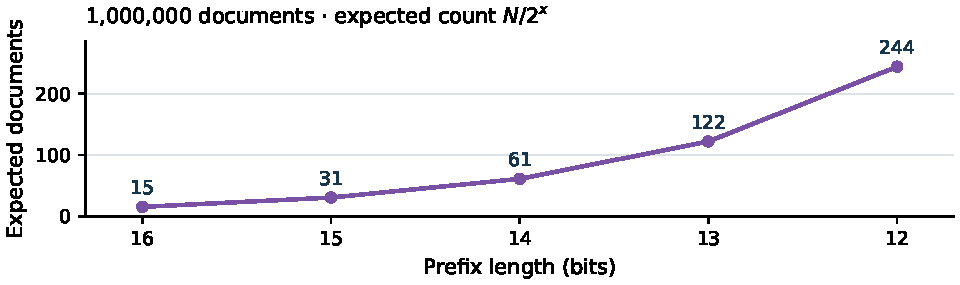
\includegraphics[width=.92\linewidth]{figures/prefix-growth.pdf}
\caption{Expected counts for one global cluster; labels are rounded. This estimates rows, not recall.}
\end{figure}

With a trie or documents ordered by their prefix, the previous range is contained inside
the parent range. We only need to process the newly introduced documents.

A simplified query algorithm becomes:

\begin{minipage}{\linewidth}
\begin{lstlisting}[language=Python]
def backward_walk(query, clusters, k, start_depth, candidate_target):
    signs = tuple(q >= 0 for q in query)
    previous = [None] * len(clusters)
    best = TopK(k)
    scored = 0
    for depth in range(start_depth, -1, -1):
        for index, cluster in enumerate(clusters):
            left, right = cluster.prefix_range(signs[:depth])
            if previous[index] is None:
                new_ranges = [(left, right)]
            else:
                old_left, old_right = previous[index]
                # Only the new rows beside the old range need scores.
                new_ranges = [(left, old_left), (old_right, right)]
            for start, stop in new_ranges:
                for row_id, code in cluster.rows_in_range(start, stop):
                    best.add(row_id, full_score(query, code))
                scored += stop - start
            previous[index] = (left, right)

        # Finish this depth in every cluster before testing the target.
        if candidate_target > 0 and scored >= candidate_target:
            break
    return best.results()
\end{lstlisting}
\end{minipage}

There is one important distinction here.

Stopping simply because we have collected, for example, 100 candidates is an approximate
stopping rule. It does not mathematically prove that a better document does not exist
outside the current prefix.

Therefore, in the experiments, recall still needs to be measured against the same exact
reference results. An exact version would require a valid upper bound on the scores of
documents outside the currently visited prefix.

\textbf{Relationship to HNSW}\par
At first glance, this approach may sound somewhat similar to HNSW because both methods use
a hierarchy to progressively change the search space.

However, the hierarchy is being used differently.

HNSW builds a proximity graph. During a query, it begins from sparse upper layers, navigates
toward promising neighbors, and progressively descends toward the denser bottom layer~\cite{hnsw}.

Backward Walk does not need to navigate between neighboring document vectors. The query
itself directly tells us where to begin:
\[
\text{query}\to\text{binary prefix}\to\text{exact prefix lookup}
\]
We then broaden that prefix only when necessary.

So conceptually:
\begin{center}\small
\begin{tabularx}{\linewidth}{@{}lYY@{}}\toprule
 & HNSW & Backward Walk\\\midrule
Index & Proximity graph & Prefix / key hierarchy\\
Query start & Sparse graph layer & Query's own binary prefix\\
Movement & Neighbor $\to$ neighbor & Specific prefix $\to$ broader prefix\\
Index insertion & Find neighbors + maintain edges & Compute prefix + insert into bucket/range\\
Search signal & Vector distance & Prefix agreement\\\bottomrule
\end{tabularx}
\end{center}

\textbf{Potential advantage 1: cheaper index construction and updates}\par
One possible advantage that I would like to investigate further is the cost of adding new documents.

For HNSW, inserting a new vector generally requires searching the existing graph to find
suitable neighbors and then creating or updating graph connections.

For Backward Walk, the conceptual insertion process is much simpler:
\[
\text{document}\to\text{embedding}\to\text{binary signs}\to\text{prefix key}\to\text{corresponding bucket}
\]
There is no nearest-neighbor graph that needs to be constructed for each new document.
So Backward Walk may be attractive for a search index that changes frequently.

I would frame this as a hypothesis to verify, because the actual insertion cost still
depends on how the buckets, ranges and on-disk/in-memory index are implemented.

\textbf{Potential advantage 2: Matryoshka prefixes give the relaxation some meaning}\par
There is also a useful connection with Matryoshka embeddings.

A Matryoshka model is trained so that shorter prefixes of the embedding remain useful
representations~\cite{mrl}.

Therefore, moving from, for example, $16\text{ bits}\to15\text{ bits}\to14\text{ bits}$
is not simply dropping arbitrary dimensions from an ordinary embedding. We are progressively
moving to shorter prefixes of a representation that was specifically trained to retain
useful information at multiple prefix lengths.

However, this does not mean that the first coordinate is always more important than the
second, or that the nearest neighbor under 16 dimensions must remain the nearest neighbor
under 15 dimensions.

Matryoshka training gives us a reason to believe that shorter prefixes remain meaningful;
the actual recall of each prefix still has to be measured.
